
\vspace*{-5pt}

\section{Experiments}
\label{sec:experiments}

We evaluate and compare the training and test performance of GIN and less powerful GNN variants.\footnote{The code is available at \url{https://github.com/weihua916/powerful-gnns.}} Training set performance allows us to compare different GNN models based on their representational power and test set performance quantifies generalization ability.

%\subsection{Settings}
{\bf Datasets.} We use 9 graph classification benchmarks: 4 bioinformatics datasets (MUTAG, PTC, NCI1, PROTEINS) and 5 social network datasets (COLLAB, IMDB-BINARY, IMDB-MULTI, REDDIT-BINARY and REDDIT-MULTI5K)~\citep{yanardag2015deep}. Importantly, our goal here is not to allow the models to rely on the input node features but mainly learn from the network structure. Thus, in the bioinformatic graphs, the nodes have categorical input features but in the social networks, they have no features. For social networks we create node features as follows: for the REDDIT datasets, we set all node feature vectors to be the same (thus, features here are uninformative); for the other social graphs, we use one-hot encodings of node degrees. Dataset statistics are summarized in Table \ref{tab:results}, and more details of the data can be found in Appendix \ref{app:dataset}. 

{\bf Models and configurations.} \revise{We evaluate GINs (Eqs.~\ref{GIN-agg} and \ref{eq:GIN-readout}) and the less powerful GNN variants. Under the GIN framework, we consider two variants: (1) a GIN that learns $\epsilon$ in \refeq{GIN-agg} by gradient descent, which we call GIN-$\epsilon$, and (2) a simpler (slightly less powerful)\footnote{There exist certain (somewhat contrived) graphs that GIN-$\epsilon$ can distinguish but GIN-0 cannot.} GIN, where $\epsilon$ in \refeq{GIN-agg} is fixed to 0, which we call GIN-0. As we will see, GIN-0 shows strong empirical performance: not only does GIN-0 fit training data equally well as GIN-$\epsilon$, it also demonstrates good generalization, slightly but consistently outperforming GIN-$\epsilon$ in terms of test accuracy.
For the less powerful GNN variants, we consider architectures that replace the sum in the GIN-0 aggregation with mean or max-pooling\footnote{For REDDIT-BINARY, REDDIT--MULTI5K, and COLLAB, we did not run experiments for max-pooling due to GPU memory constraints.}, or replace MLPs with 1-layer perceptrons, {\ie}, a linear mapping followed by ReLU.}
In Figure~\ref{fig:curve} and Table~\ref{tab:results}, a model is named by the aggregator/perceptron it uses. Here mean--1-layer and max--1-layer correspond to GCN and GraphSAGE, respectively, up to minor architecture modifications. We apply the same graph-level readout (READOUT in \refeq{eq:GIN-readout}) for GINs and all the GNN variants, specifically, sum readout on bioinformatics datasets and mean readout on social datasets due to better test performance.

Following \citep{yanardag2015deep, niepert2016learning}, we perform 10-fold cross-validation with LIB-SVM \citep{chang2011libsvm}. \revise{We report the average and standard deviation of validation accuracies across the 10 folds within the cross-validation.}
For all configurations, 5 GNN layers (including the input layer) are applied, and all MLPs have $2$ layers. Batch normalization \citep{ioffe2015batch} is applied on every hidden layer. We use the Adam optimizer \citep{kingma2014adam} with initial learning rate $0.01$ and decay the learning rate by $0.5$ every 50 epochs. The hyper-parameters we tune for each dataset are: (1) the number of hidden units $\in \{16, 32\}$ for bioinformatics graphs and $64$ for social graphs; (2) the batch size $\in \{32, 128\}$; (3) the dropout ratio $\in \{0, 0.5\}$ after the dense layer \citep{srivastava2014dropout}; (4) the number of epochs, \ie, a single epoch with the best cross-validation accuracy averaged over the 10 folds was selected. Note that due to the small dataset sizes, an alternative setting, where hyper-parameter selection is done using a validation set, is extremely unstable, \eg, for MUTAG, the validation set only contains 18 data points.
We also report the training accuracy of different GNNs, where all the hyper-parameters were fixed across the datasets: 5 GNN layers (including the input layer), hidden units of size 64, minibatch of size 128, and 0.5 dropout ratio. For comparison, the training accuracy of the WL subtree kernel is reported, where we set the number of iterations to 4, which is comparable to the 5 GNN layers.


{\bf Baselines.}
We compare the GNNs above with a number of state-of-the-art baselines for graph classification: 
(1) the WL subtree kernel \citep{shervashidze2011weisfeiler}, where $C$-SVM \citep{chang2011libsvm} was used as a classifier; the hyper-parameters we tune are $C$ of the SVM and the number of WL iterations $\in \{1, 2, \ldots, 6\}$; (2) state-of-the-art deep learning architectures, i.e., Diffusion-convolutional neural networks (DCNN)~\citep{atwood2016diffusion}, PATCHY-SAN \citep{niepert2016learning} and Deep Graph CNN (DGCNN) \citep{zhang2018end}; (3) Anonymous Walk Embeddings (AWL) \citep{ivanov2018anonymous}. For the deep learning methods and AWL, we report the accuracies reported in the original papers.


\begin{figure}[t]
 \vspace{-0.15in}
    \centering
        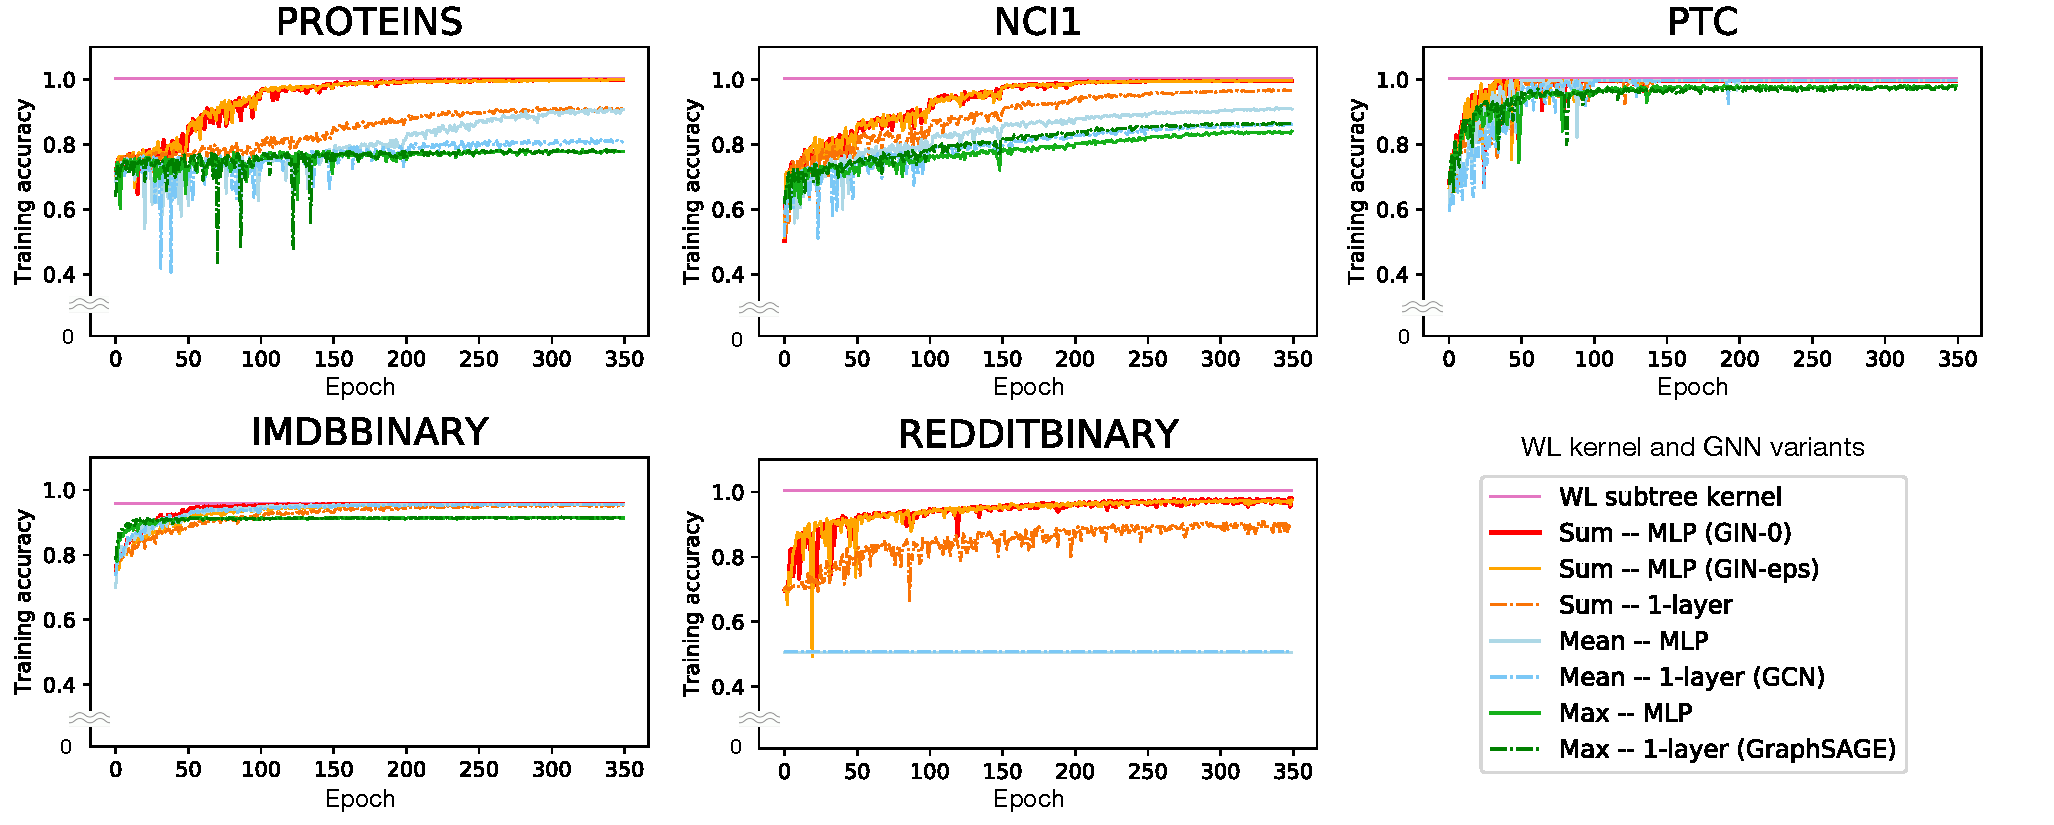
\includegraphics[width=\textwidth]{learning_curve.pdf}   
    \caption{Training set performance of GINs, less powerful GNN variants, and the WL subtree kernel. 
    %\jure{This should go to the main text:} 
    %\jure{which of these is GraphSAGe, which is GCN. Let's say/label them.}
    }
    \label{fig:curve}
\end{figure}

\begin{table}[t]\
\resizebox{1.0\textwidth}{!}{ \renewcommand{\arraystretch}{1.25}
\centering
\begin{tabular}{@{}clcccccccccc@{}}\cmidrule[\heavyrulewidth]{2-12}
%& \multirow{3}{*}{\vspace*{8pt}\textbf{Method}}&\multicolumn{5}{c}{\textbf{Dataset}}\\\cmidrule{3-7}
& Datasets &  {\textsc{IMDB-B}} & {\textsc{IMDB-M}}  & {\textsc{RDT-B}} & {\textsc{RDT-M5K}} & {\textsc{COLLAB}} & {\textsc{MUTAG}} &  {\textsc{PROTEINS}}  & {\textsc{PTC}} & {\textsc{NCI1}}  \\
%\\ \cmidrule{2-7}  
\multirow{3}{*}{\rotatebox{90}{\hspace*{+3pt}Datasets}}
& \text{\# graphs }  & 1000  & 1500  & 2000  &  5000 & 5000 &    188 & 1113 & 344  &  4110     \\
& \text{\# classes }   &  2  & 3  & 2  &  5 &  3 &  2 & 2  &  2   & 2 \\
& \text{Avg \# nodes }  &  19.8   & 13.0  & 429.6  &  508.5 &  74.5 &  17.9 & 39.1  & 25.5  &  29.8  
\\ \cmidrule{2-12}
\multirow{5}{*}{\rotatebox{90}{\hspace*{-10pt}Baselines}}        
& \text{WL subtree}         &  73.8 $\pm$ 3.9   & 50.9 $\pm$ 3.8   & 81.0 $\pm$ 3.1  &  52.5 $\pm$ 2.1  &  78.9 $\pm$ 1.9 & 90.4 $\pm$ 5.7     & 75.0 $\pm$ 3.1   & 59.9 $\pm$ 4.3 &  {\bf 86.0 $\pm$ 1.8} $^\ast$  \\
& \textsc{DCNN}             &  49.1 & 33.5     &  -- & -- & 52.1 &  67.0 & 61.3 & 56.6 &  62.6 \\
& \textsc{PatchySan}        & 71.0 $\pm$ 2.2  & 45.2 $\pm$ 2.8  & 86.3 $\pm$ 1.6  &  49.1 $\pm$ 0.7 & 72.6 $\pm$ 2.2 & {\bf 92.6 $\pm$ 4.2} $^\ast$  & 75.9 $\pm$ 2.8  & 60.0 $\pm$ 4.8   &  78.6 $\pm$ 1.9     \\ 
& \textsc{DGCNN}           & 70.0 &  47.8    & --   & --     & 73.7 & 85.8        &  75.5   & 58.6  & 74.4   \\ 
& \textsc{AWL}               & 74.5 $\pm$ 5.9  & 51.5 $\pm$ 3.6    & 87.9 $\pm$ 2.5 & 54.7 $\pm$ 2.9    & 73.9 $\pm$ 1.9    & 87.9 $\pm$ 9.8        & -- & --  & --  \\ \cmidrule{2-12}
\multirow{6}{*}{\rotatebox{90}{\hspace*{-10pt}GNN variants}} 
& \textsc{Sum--MLP ({\bf GIN-0)}}   &  {\bf 75.1 $\pm$ 5.1}     & {\bf 52.3 $\pm$ 2.8}    &  {\bf 92.4 $\pm$ 2.5}             &  {\bf 57.5 $\pm$ 1.5}             & {\bf 80.2 $\pm$ 1.9}      &  {\bf 89.4 $\pm$ 5.6}     & {\bf 76.2 $\pm$ 2.8}    & {\bf 64.6 $\pm$ 7.0}  & {\bf 82.7 $\pm$ 1.7}   \\
& \textsc{Sum--MLP ({\bf GIN-$\epsilon$}})   &  {\bf 74.3 $\pm$ 5.1}     & {\bf 52.1 $\pm$ 3.6}    &  {\bf 92.2 $\pm$ 2.3}             &  {\bf 57.0 $\pm$ 1.7}             & {\bf 80.1 $\pm$ 1.9}      &  {\bf 89.0 $\pm$ 6.0}     & {\bf 75.9 $\pm$ 3.8}    & 63.7 $\pm$ 8.2  & {\bf 82.7 $\pm$ 1.6}   \\
& \textsc{Sum--1-Layer}     &  74.1 $\pm$ 5.0    & {\bf 52.2 $\pm$ 2.4}    &  90.0 $\pm$ 2.7        &  55.1 $\pm$ 1.6            & {\bf 80.6 $\pm$ 1.9}      &  {\bf 90.0 $\pm$ 8.8}     & {\bf 76.2 $\pm$ 2.6}     & 63.1 $\pm$ 5.7 & 82.0 $\pm$ 1.5  \\
%& \textsc{Mean--MLP}       &  73.7 $\pm$ 3.7  & {\bf 52.3 $\pm$ 3.1}     &  \begin{tabular}{c} 50.0$\pm$ 0.0 $^{\dagger}$  \\(71.2 $\pm$ 4.6) \end{tabular}  &  \begin{tabular}{c} 20.0 $\pm$ 0.0 $^{\dagger}$ \\ (41.3 $\pm$ 2.1)\end{tabular} & 79.2 $\pm$ 2.3      &  83.5 $\pm$ 6.3        & 75.5 $\pm$ 3.4     & {\bf 66.6 $\pm$ 6.9}  & 80.9 $\pm$ 1.8  \\ 
%& \textsc{Mean--1-Layer} (GCN)  &  74.0 $\pm$ 3.4    & 51.9 $\pm$ 3.8  &  \begin{tabular}{c} 50.0 $\pm$ 0.0 $^{\dagger}$ \\  (69.7 $\pm$ 3.2) \end{tabular} &  \begin{tabular}{c} 20.0 $\pm$ 0.0 $^{\dagger}$\\ (39.7 $\pm$ 2.4) \end{tabular} & 79.0 $\pm$ 1.8               & 85.6 $\pm$ 5.8     & 76.0 $\pm$ 3.2     & 64.2 $\pm$ 4.3  & 80.2 $\pm$ 2.0   & \\
& \textsc{Mean--MLP}       &  73.7 $\pm$ 3.7  & {\bf 52.3 $\pm$ 3.1}     & 50.0 $\pm$ 0.0  &  20.0 $\pm$ 0.0 & 79.2 $\pm$ 2.3      &  83.5 $\pm$ 6.3        & 75.5 $\pm$ 3.4     & {\bf 66.6 $\pm$ 6.9}  & 80.9 $\pm$ 1.8  \\ 
& \textsc{Mean--1-Layer} (GCN)  &  74.0 $\pm$ 3.4    & 51.9 $\pm$ 3.8  & 50.0 $\pm$ 0.0  &  20.0 $\pm$ 0.0 & 79.0 $\pm$ 1.8               & 85.6 $\pm$ 5.8     & 76.0 $\pm$ 3.2     & 64.2 $\pm$ 4.3  & 80.2 $\pm$ 2.0   & \\   
& \textsc{Max--MLP}  &  73.2 $\pm$ 5.8    & 51.1 $\pm$ 3.6    &  --                       &  --                      &      --              & 84.0 $\pm$ 6.1          & 76.0 $\pm$ 3.2   & 64.6 $\pm$ 10.2 & 77.8 $\pm$ 1.3  & \\ 
& \textsc{Max--1-Layer} (GraphSAGE)    &  72.3 $\pm$ 5.3           & 50.9 $\pm$ 2.2    &  --                         &  --                      &      --                    & 85.1 $\pm$ 7.6  & 75.9 $\pm$ 3.2 & 63.9 $\pm$ 7.7 & 77.7 $\pm$ 1.5 & \\         
\cmidrule[\heavyrulewidth]{2-12}
\end{tabular}}
 \caption{{\bf Test set classification accuracies (\%).} 
 %$^{\dagger}$ indicate test accuracies (equal to chance rates) when all nodes have the same feature vector. We also report in the parentheses the test accuracies when the node degrees are used as input node features. 
 The best-performing GNNs are highlighted with boldface. On datasets where GINs' accuracy is not strictly the highest among GNN variants, we see that GINs are still comparable to the best GNN because a paired t-test at significance level 10\% does not distinguish GINs from the best; thus, GINs are also highlighted with boldface. If a baseline performs significantly better than all GNNs, we highlight it with boldface and asterisk.
%\jure{Is there a really good reason that we are including $^{\dagger}$ and $()$. Can we just pick one -- in the main text we say that in reddit we use all node feature vectors to be the same. So let's jut go with that and that's ok and simplify the table.\\
%Also, which of these variants is GCN, which is GraphSAGE (can we explicitly label them as such)}
 }
  \label{tab:results}
  \vspace{-0.1in}
\end{table}


\subsection{Results}

{\bf Training set performance.}
We validate our theoretical analysis of the representational power of GNNs by comparing their training accuracies. Models with higher representational power should have higher training set accuracy.
Figure \ref{fig:curve} shows training curves of GINs and less powerful GNN variants with the same hyper-parameter settings. 
\revise{First, both the theoretically most powerful GNN, {\ie} GIN-$\epsilon$ and GIN-0, are able to almost perfectly fit all the training sets. In our experiments, explicit learning of $\epsilon$ in GIN-$\epsilon$ yields no gain in fitting training data compared to fixing $\epsilon$ to 0 as in GIN-0.} In comparison, the GNN variants using mean/max pooling or 1-layer perceptrons severely underfit on many datasets. In particular, the training accuracy patterns align with our ranking by the models' representational power: GNN variants with MLPs tend to have higher training accuracies than those with 1-layer perceptrons, and GNNs with sum aggregators tend to fit the training sets better than those with mean and max-pooling aggregators. 

On our datasets, training accuracies of the GNNs never exceed those of the WL subtree kernel. This is expected because GNNs generally have lower discriminative power than the WL test. For example, on IMDBBINARY, none of the models can perfectly fit the training set, and the GNNs achieve at most the same training accuracy as the WL kernel. This pattern aligns with our result that the WL test provides an upper bound for the representational capacity of the aggregation-based GNNs. However, the WL kernel is not able to learn how to combine node features, which might be quite informative for a given prediction task as we will see next. %Our theoretical results focus on representational power and do not yet take into account optimization (\eg, local minima). Nonetheless, the empirical results align very well with our theory.


{\bf Test set performance.}
Next, we compare test accuracies. Although our theoretical results do not directly speak about the generalization ability of GNNs, it is reasonable to expect that GNNs with strong expressive power can accurately capture graph structures of interest and thus generalize well. Table \ref{tab:results} compares test accuracies of GINs (Sum--MLP), other GNN variants, as well as the state-of-the-art baselines.

First, GINs, \revise{especially GIN-0}, outperform (or achieve comparable performance as) the less powerful GNN variants on all the 9 datasets, achieving state-of-the-art performance. 
GINs shine on the social network datasets, which contain a relatively large number of training graphs. 
For the Reddit datasets, all nodes share the same scalar as node feature. %the same one-dimensional vector was used as node features.
Here, GINs and sum-aggregation GNNs accurately capture the graph structure and significantly outperform other models. Mean-aggregation GNNs, however, fail to capture any structures of the unlabeled graphs (as predicted in Section~\ref{sec:confuse}) and do not perform better than random guessing. Even if node degrees are provided as input features, mean-based GNNs perform much worse than sum-based GNNs (the accuracy of the GNN with mean--MLP aggregation is 71.2$\pm$4.6\% on REDDIT-BINARY and 41.3$\pm$2.1\% on REDDIT-MULTI5K).
\revise{Comparing GINs (GIN-0 and GIN-$\epsilon$), we observe that GIN-0 slightly but consistently outperforms GIN-$\epsilon$. Since both models fit training data equally well, the better generalization of GIN-0 may be explained by its simplicity compared to GIN-$\epsilon$.}
